\documentclass{scrartcl}			% defines the kind of document you want to produce

% Include different packages:
\usepackage[utf8]{inputenc}
\usepackage[T1]{fontenc}
\usepackage{lmodern}
\usepackage[english]{babel}
\usepackage{amsmath}
\usepackage{graphicx}           	% include graphics
\usepackage{caption}	
\usepackage{subcaption}	 
\usepackage{hyperref}
\usepackage{epstopdf}

\title{Neuroprothetik Exercise 1 \\ Programming Basics}
\author{ Laura Bielenberg }
\date{10. Mai 2019}


\begin{document} 					% Document begins here

\maketitle

\section{Generate a Signal}		% start a new section 

The task is to create a function that generates a signal consisting of multiple arbitrary frequency components. Inputs should be:

\begin{itemize}
\item An array of frequencies (in Hz)
\item An array of corresponding amplitudes
\item A signal offset
\item A signal duration (in seconds)
\item A sample rate (in Hz)
\end{itemize}

\subsection{Plot the Signal}		% start a new subsection

Use this function to generate a one second long signal consisting of the frequency components 100 Hz, 600 Hz and 9 kHz with the amplitudes 1, 1.5 and 2 as well as an offset of 3 and a sampling rate of 100 kHz. A plot of the first 100 ms of this 1 s long signal can be seen in figure \ref{fig:signalPlot}.
\newpage
\begin{figure}[h!]					%start figure-environment
	\centering
	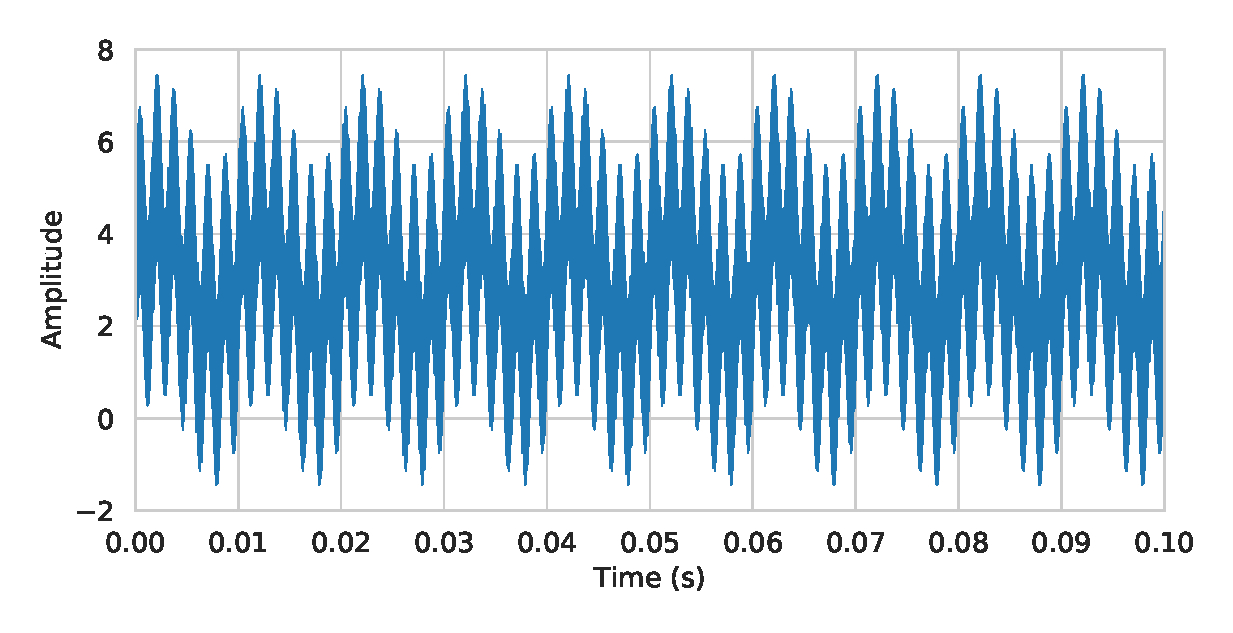
\includegraphics[width=\textwidth]{imgs/signalDataPlot.eps}
	\captionsetup{width=\textwidth}  %choose the with of the caption
	\caption{First 100 ms of the created signal with a sampling-frequency of 100 kHz.}
	\label{fig:signalPlot} %choose a label, see subsection references
\end{figure}

\newpage

\section{Calculate the Spectrum}
a) The task is to calculate the single sided amplitude spectrum of the signal created in task one using the Fast Fourier Transformation. Plots of the FFT results for signal sample rates of 100 kHz, 20 kHz and 10 kHz are given in figures \ref{fig:100kHz} to \ref{fig:10kHz}. 

\begin{figure}[h!]					%start figure-environment
	\centering
	\includegraphics[width=\textwidth]{imgs/100kHz_samplefreq.eps}
	\captionsetup{width=\textwidth}  %choose the with of the caption
	\caption{FFT for the signal shown in figure \ref{fig:signalPlot} for a sampling frequency of 100 kHz. Only frequencies up to 10 kHz are shown.}
	\label{fig:100kHz} %choose a label, see subsection references
\end{figure}

\begin{figure}[h!]					%start figure-environment
	\centering
	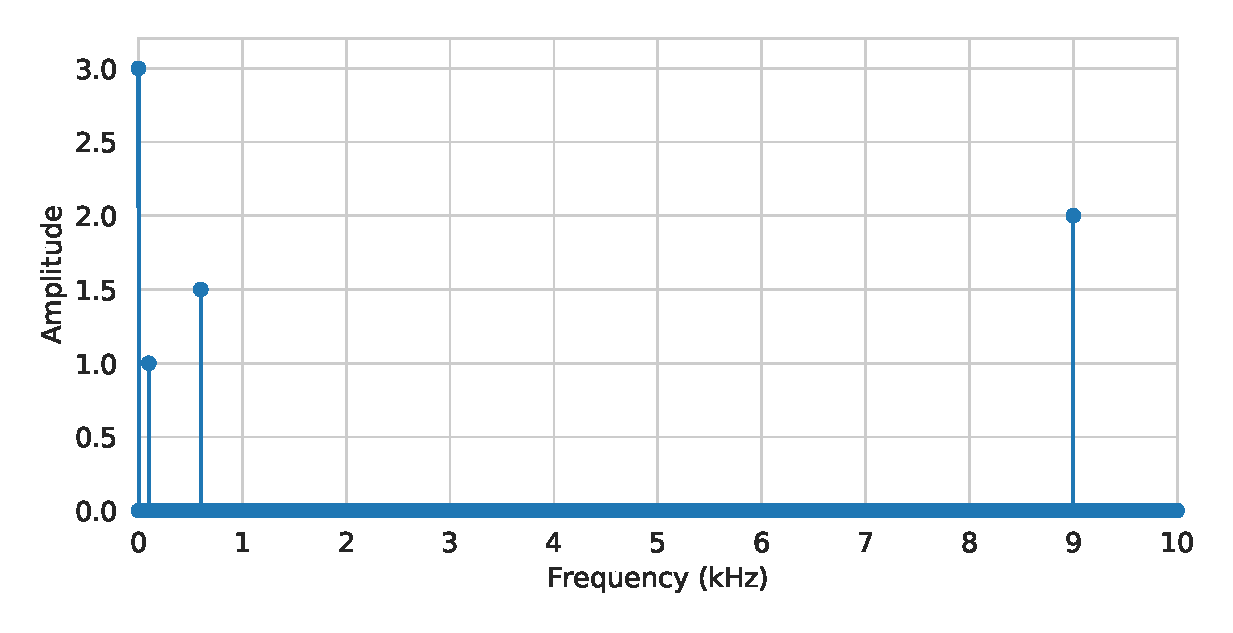
\includegraphics[width=\textwidth]{imgs/20kHz_samplefreq.eps}
	\captionsetup{width=\textwidth}  %choose the with of the caption
	\caption{FFT for a sampling frequency of 20 kHz.}
	\label{fig:20kHz} %choose a label, see subsection references
\end{figure}

\begin{figure}[h!]					%start figure-environment
	\centering
	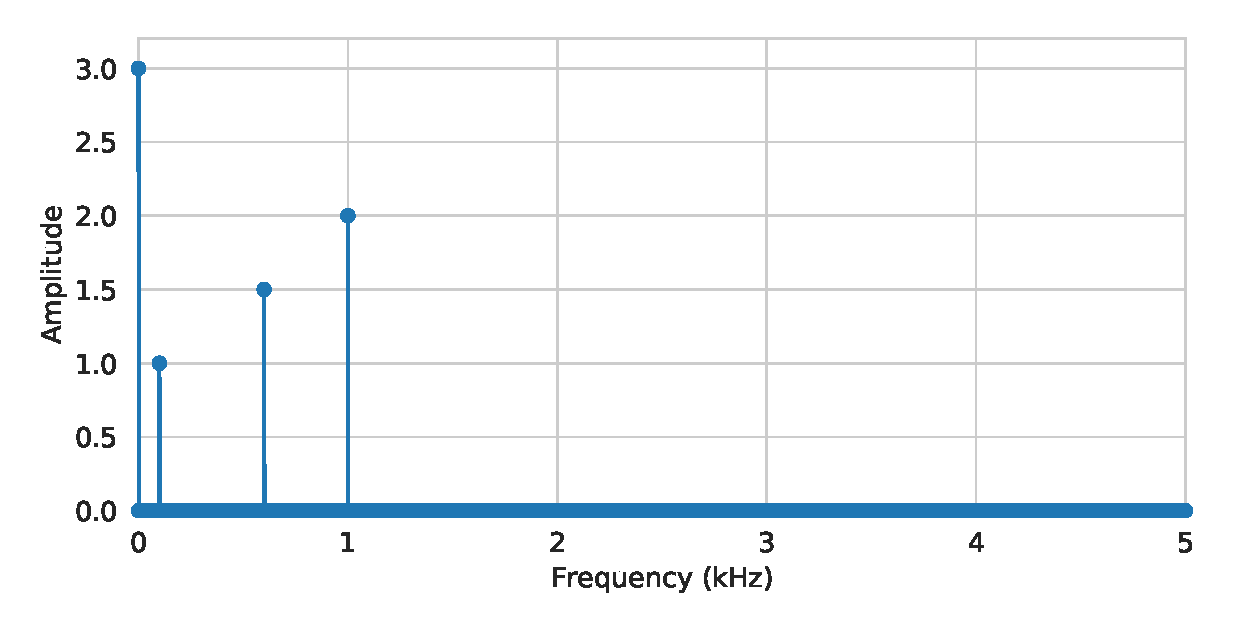
\includegraphics[width=\textwidth]{imgs/10kHz_samplefreq.eps}
	\captionsetup{width=\textwidth}  %choose the with of the caption
	\caption{FFT for a sampling frequency of 10 kHz.}
	\label{fig:10kHz} %choose a label, see subsection references
\end{figure}
b) Explain what you see in these spectra and what measure would be necessary to perform a fft on the given signals and still obtain correct values.\\
\newline
The spectra show the frequencies of which the signal is composed, and their corresponding amplitudes. The first peek at 0 Hz is due to the signal offset. While the FFTs for sampling frequencies of 100 kHz and 20 kHz show the expected frequency bands at 100 Hz, 600 Hz and 9 kHz the plot for a sampling frequency of 10 kHz shows an additional peek at 1 kHz. The reason for this is, that by using a sampling frequency of only 10 kHz, the Nyquist Theorem, by which the sampling frequency has to be at least twice as big as the largest signal frequency, is not fulfilled. Therefore the higher frequencies of the signal are not sampled correctly. 
\end{document}